\documentclass[10pt,a4paper,oneside]{book}

\usepackage[utf8]{inputenc}
\usepackage[T1]{fontenc}
\usepackage[french]{babel}
%\renewcommand\sfdefault{phv}
\usepackage[left=2cm, right=2cm, bottom=1.85cm, top=1.5cm]{geometry}

\usepackage{fancyhdr}
\usepackage{framed}
\pagestyle{fancy}
\usepackage{hyperref}
%\renewcommand{\headrulewidth}{1pt}
%\fancyhead[C]{\textbf{page \thepage}} 
\fancyhead[L]{Cours}
\fancyhead[R]{Seconde}
\usepackage[skip=15pt plus1pt, indent=15pt]{parskip}

\renewcommand{\footrulewidth}{1pt}
\fancyfoot[C]{\textbf{page \thepage}} 
\fancyfoot[L]{Lycée Jacques Brel}
\fancyfoot[R]{Année 2022-2023}



\usepackage{pgfplots}

\pgfplotsset{compat=newest}
\pgfplotsset{every axis/.append style={
                    axis x line=middle,
                    axis y line=middle,
                    axis line style={->},
                    xlabel={$x$},
                    ylabel={$y$},
                    label style={font=\scriptsize},
                    tick label style={font=\tiny},
                    unit vector ratio*=1 1 1,
   					xlabel style={at={(ticklabel* cs:1)},anchor=north west},
   					ylabel style={at={(ticklabel* cs:1)},anchor=south west}
                    }}


%%%%%%%%%%%%%%%%%%%%%%%%%%%%%%%%%%%%%%%%%%%%%%%%%%

%\newcommand{\TDoc}[1]{
%\begin{center}
%{\setlength{\fboxsep}{10pt}  % Ecart texte-boite
%\shadowbox{\textbf{\Large{#1}}}}
%\end{center}
%\vspace{1.5cm}}
    
 \usepackage{fancybox}   %pour l'encadré du titre shadowbox
 \usepackage{stmaryrd}   %pour utiliser correctement les crochets pour les ensembles de définitions
 \usepackage[normalem]{ulem}
 \usepackage{graphicx}
 %\usepackage{wrapfig} %texte coulé autour d'une image
 \usepackage{soul} % souligné
 \usepackage{nonfloat}
 \usepackage[standard]{ntheorem}
 \usepackage{array}
 \usepackage{arydshln}
 \usepackage{graphicx}
%MATHEMATIQUES
\usepackage{amsmath,amsfonts} 

\usepackage{tikz}
\newcommand{\N}{\mathbb{N}}
\newcommand{\Z}{\mathbb{Z}}
\newcommand{\D}{\mathbb{D}}
\newcommand{\Q}{\mathbb{Q}}
\newcommand{\R}{\mathbb{R}}
\newcommand{\Co}{\mathbb{C}}
\newcommand{\K}{\mathbb{K}}
\newcommand{\F}{\mathbb{F}}

%%%%% Tableaux de variations
\usepackage{tkz-tab}
%%%%%

%%%%%%%%%%%%%%%%%%%%%%%%%%%%%%%%%%%

\makeatletter
%%%%%%%%%%%%%%%%%%% debut fichier boiboites.sty %%%%%%%%%%%%%%%%%%%%%%
\RequirePackage{xkeyval}
\RequirePackage{tikz}
\usetikzlibrary{intersections}
\usetikzlibrary{positioning}
\usetikzlibrary{3d}
\RequirePackage{amssymb}

\define@key{boxedtheorem}{titlecolor}{\def\titlecolor{#1}}
\define@key{boxedtheorem}{titlebackground}{\def\titlebackground{#1}}
\define@key{boxedtheorem}{background}{\def\background{#1}}
\define@key{boxedtheorem}{titleboxcolor}{\def\titleboxcolor{#1}}
\define@key{boxedtheorem}{boxcolor}{\def\boxcolor{#1}}
\define@key{boxedtheorem}{thcounter}{\def\thcounter{#1}}
\define@key{boxedtheorem}{size}{\def\size{#1}}
\presetkeys{boxedtheorem}{titlecolor = black, titlebackground = white, background = white,%
                         titleboxcolor = black, boxcolor = black, thcounter=, size = .9\textwidth}{}

\newcommand{\couleurs}[1][]{%
    \setkeys{boxedtheorem}{#1}
    \tikzstyle{fancytitle} =[draw=\titleboxcolor, rounded corners, fill=\titlebackground,
                            text= \titlecolor]
    \tikzstyle{mybox} = [draw=\boxcolor, fill=\background, very thick,
                        rectangle, rounded corners, inner sep=10pt, inner ysep=20pt]
}


%Commande generique pour faire un joli encadre
\newsavebox{\boiboite}
\newcommand{\titre}{Titre}
\newenvironment{boite}[2][]%
    {%
    \renewcommand{\titre}{#2}
    \couleurs[#1]
    \begin{lrbox}{\boiboite}%
     \begin{minipage}[!h]{\size}
    }%
    {%
     \end{minipage}
    \end{lrbox}
    \begin{center}
    \begin{tikzpicture}
    \node [mybox] (box){\usebox{\boiboite}};
    \node[fancytitle, right=10pt] at (box.north west) {\titre};
    \end{tikzpicture}
    \end{center}
    }

\newcommand{\newboxedtheorem}[4][]{%
    \couleurs[#1]
    \@ifnotempty{#4}{%
      \@ifundefined{the#4}{\@ifundefined{\thcounter}{\newcounter{#4}}{%
      \newcounter{#4}[\thcounter ] } } { }%
    }
    \newenvironment{#2}[1][]{%
    \@ifnotempty{#4}{\refstepcounter{#4}}
    \begin{boite}[#1]{\textbf{#3\@ifnotempty{#4}{ \csname the#4\endcsname}}\@ifnotempty{##1}{
    (##1)}}
    }%
    {%
    \end{boite}
    }
}

\newcommand{\newboxedtheoreme}[4][]{%
    \couleurs[#1]
    \@ifnotempty{#4}{%
      \@ifundefined{the#4}{\@ifundefined{}{}{%
      } } { }%
    }
    \newenvironment{#2}[1][]{%
    \@ifnotempty{#4}{\refstepcounter{#4}}
    \begin{boite}[#1]{\textbf{#3\@ifnotempty{#4}{ \csname the#4\endcsname}}\@ifnotempty{##1}{
    (##1)}}
    }%
    {%
    \end{boite}
    }
}
%%%%%%%%%%%%%%%%%%%% end fichier boiboites.sty %%%%%%%%%%%%%%%%%%%%%%


\newboxedtheorem{theo}{Théorème}{theorem}
\newboxedtheorem{de}{D\'efinition}{theorem}
\newboxedtheorem{prop}{Propriété}{theorem}
\newboxedtheorem{pro}{Proposition}{theorem}
\newboxedtheorem{nota}{Notation}{theorem}
\newtheorem{exo}{Exercice}
\newboxedtheorem{exe}{Exemple}{theorem}
\newboxedtheorem{cor}{Corolaire}{theorem}
\newboxedtheoreme{conc}{Conclusion}{theorem*}
\newboxedtheoreme{demo}{\textbf{Démonstration guidée}}{theorem}
%%%%%%%%%%%%%%%%%%%%%%%%%%%%%%
%%%%%%%%%%%%%%%%%%%%%%%%%%%%%
\newlength{\longA}
\newlength{\longB}
\newenvironment{BoiteShadow}[3][\linewidth]{%
\addtolength{\longA}{#2}
\addtolength{\longB}{#3}
\begin{Sbox}\begin{minipage}{#1}}%
{\end{minipage}\end{Sbox}%
\setlength{\fboxsep}{\longA}
\setlength{\shadowsize}{\longB}
\shadowbox{\unhbox\@Sbox}\par}
\makeatother
%\author{Augustin WENGER}

\title{Cours de Seconde 1 2022-2023}
\date{}

%%%% fin du préambule, on passe au contenu : tout le texte entre
%%%% \begin{document} et \end{document} 

\begin{document}
\maketitle
\tableofcontents
\chapter{Ensembles de nombres}

\section{Ensemble : vocabulaire et notations}

\begin{de}
    Un \underline{ensemble} est une collection d'objets, appelés \underline{éléments}, qu'il contient. 
\end{de}

Quand on peut décrire tous les éléments contenus dans un ensemble, on peut noter ces éléments séparés par des points-virgules (ou des virgules si on ne peut pas prendre les éléments pour des nombres décimaux) entre des $\{\}$

Exemples : 
\begin{itemize}
    \item L'ensemble des nombres premiers plus petits que $10$ est $\{2;3;5;7\}$
    \item L'ensemble qui ne contient aucun élément s'appelle l'ensemble vide et est noté $\emptyset$
    \item L'ensemble des jours de la semaine peut être noté $\{lundi, mardi, mercredi, jeudi, vendredi, samedi, dimanche\}$  (On peut faire des ensembles d'autre chose que de nombres)
\end{itemize}


\begin{de}
    Si un élément est contenu dans un ensemble, on dit qu'il \underline{appartient} à cet ensemble, que l'on note $\in$.
    Si un élément n'appartient pas à un ensemble, on note $\notin$ 
\end{de}



Exemples : 
\begin{itemize}
    \item $2 \in \{2;3;5;7\}$ 
    \item $4 \notin \{2;3;5;7\}$
    \item $\{2;7\} \notin \{2;3;5;7\}$  (L'ensemble de droite contient des nombres, pas des ensembles)
    \item Cette notation avait déjà été vue en $6$-ème : on disait qu'un point appartient à une droite. En effet, une droite est un ensemble de points (des ensembles de points qui vérifient une certaine équation, cf les équations de droite)
    \item On a $A=\{2;3;5;9\}$, $B=\{0;1;2;3;4;5;6;7;8;9\}$ et $C=\{1;12\}$ alors $A\subset B$ 
  et mais $C$ n'est pas inclus dans $B$, ni dans $A$.
\end{itemize}

Remarques : 
\begin{itemize}
\item Un ensemble est entièrement caractérisé par les éléments qu'il contient. Deux ensembles contenant exactement les mêmes éléments sont égaux. Ainsi, l'ordre des éléments n'importe pas dans un ensemble et on pourrait aussi noter $\{7;2;5;3\}$ au lieu de $\{2;3;5;7\}$
\item Comme tous les objets mathématiques, on peut donner un nom à un ensemble pour généraliser ou l'écrire plus rapidement. Par exemple si on note $E$ l'ensemble $\{2;3;5;7\}$, $2 \in E$
\end{itemize}


\begin{de}
     Si un ensemble $E$ contient exclusivement des éléments contenus dans un autre ensemble $F$, on dit que $E$ est \underline{inclus} dans $F$ et l'on note $E \subset F$.
\end{de}

Remarques :
\begin{itemize}
    \item Si un ensemble $E$ n'est pas inclus dans un ensemble $F$, on écrit $E \not\subset F$
    \item Comme pour le signe $<$, le signe $\subset$ se transmet dans le sens où Si E est inclus dans F qui est inclus dans G, alors E est inclus dans G. Ou sous la forme de formule : Si $E \subset F$ et $F \subset G$, alors $E \subset G$. On dit que \textit{la relation d'inclusion est transitive}
\end{itemize}
    

Exemples : 
\begin{itemize}
    \item $\{2;7\} \subset \{2;3;5;7\}$
    \item $\{2;7;9\} \not\subset \{2;3;5;7\}$
    \item Un ensemble $E$ est toujours par définition inclus dans lui même : $E \subset E$.
    \item Attention : ne jamais écrire $2 \subset \{2;3;5;7\}$, $2$ est un élément qui appartient à l'ensemble, mais seul un ensemble peut-être inclus dans un autre. Il faudrait écrire $\{2\} \subset \{2;3;5;7\}$ ou $2 \in \{2;3;5;7\}$
\end{itemize}

On peut dessiner des ensembles, on appelle cela des diagrammes de Venn. On représente souvent deux ensembles inclus l'un dans l'autre par deux sacs inclus l'un dans l'autre, comme dans la figure \ref{fig:Ensembles}



\begin{exo}
    \begin{itemize}
        \item Représenter graphiquement sous forme de diagramme de Venn (en respectant les inclusions) les ensembles suivants :
        \begin{itemize}
            \item Mammifères
            \item Canidés
            \item Animaux
            \item Chiens
            \item Chats
        \end{itemize}
    \item Placez correctement dans les ensembles les animaux suivants :
        \begin{itemize}
            \item Hélène la baleine
            \item Igor le labrador
            \item Sacha le chat
            \item Edgar le renard
            \item Miche-Miche le caniche
            \item Régine la sardine
    \item Dites si les expressions suivantes sont vraies ou fausses :
        \begin{itemize}
            \item Igor $\in$ Chiens
            \item Régine $\in$ Chats
            \item Igor $\in$ Canidés
            \item Chats $\subset$ Mammifères
            \item Mammifères $\not\subset$ Chiens
            \item Chats $\subset$ Mammifères
        \end{itemize} 
        \end{itemize}    
    \end{itemize}
\end{exo}



\section{Les ensembles de nombres}
Les nombres utilisés en mathématiques, suivant leurs caractéristiques, sont regroupés 
dans des ensembles. On distingues six grandes familles de nombres:
\subsection{Les entiers naturels $\N$}
Les entiers naturels sont les nombres entiers positifs c'est à dire, en notant $\N$ 
(notation) l'ensemble des entiers naturels, on a:

$$\N=\{0;1;2;3;\cdots\}$$
\subsection{Les entiers relatifs $\Z$}
Les entiers relatifs sont les nombres entiers positifs ou négatifs c'est à dire, en notant $\Z$ 
(notation) l'ensemble des entiers relatifs, on a:
$$\Z=\{\cdots;-3;-2;-1;0;1;2;3;\cdots\}$$

\subsection{Les nombres décimaux $\D$}
Les nombres décimaux sont les nombres qui s'écrivent avec un nombre fini de chiffres après la virgule,
 c'est à dire, en notant $\D$ 
(notation) l'ensemble des nombres décimaux, on a:
$$\D=\{\cdots;-0{,}5;-16{,}15;0;1{,}125;2{,}4567;3{,}00017;\cdots\}$$
Remarque : les nombres entiers sont tous des nombres décimaux : ils ont zéro chiffres après la virgule, ce qui rentre bien dans la définition notée plus haut.
\begin{prop}
  Un nombre $x\in\D$ si et seulement il existe $n\in\N$ tel que $x\times 10^{n}\in\Z$.
\end{prop}
Cette propriétée signifie que tout nombre décimal $x$ peut s'écrire sous la forme: 
$$x=\frac{a}{10^{n}}$$
Où $a\in\Z$. De plus, tout nombre pouvant s'écrire sous cette forme est décimal.

\subsection{Les nombres rationnels $\Q$}
Les nombres rationnels sont les quotients d'entiers relatifs, c'est à dire, en notant $\Q$ 
(notation) l'ensemble des nombres rationnels, on a:


$$\Q=\{\cdots;-\frac{7}{5};-\frac{1}{3};-\frac{12}{151};0;\frac{17}{13};\frac{2}{7};\frac{3}{8};\cdots\}$$

Remarque : Les nombres décimaux sont tous des nombres rationnels, puisque l'on a vu que tout nombre décimal pouvait s'écrire comme une fraction d'entiers.

\subsection{Les nombres réels $\R$}

Les nombres réels sont tous les nombres, c'est à dire, en notant $\R$ 
(notation) l'ensemble des nombres réels, $\R$ contient tous les nombres cités précédement et aussi ceux 
qui n'entrent pas dans les familles précédentes (qu'on appelle nombres irrationnels). On a:

$$\R=\{\cdots;-\frac{7}{5};-\frac{\pi}{3};-\frac{12}{\sqrt{2}};0;\sqrt{3};\pi;127;\cdots\}$$

On peut remarquer les inclusions suivantes:
$$\N\subset\Z\subset\D\subset\Q\subset\R$$
On peut aussi visualiser cela ainsi:



\begin{figure}[htbp]
\centering
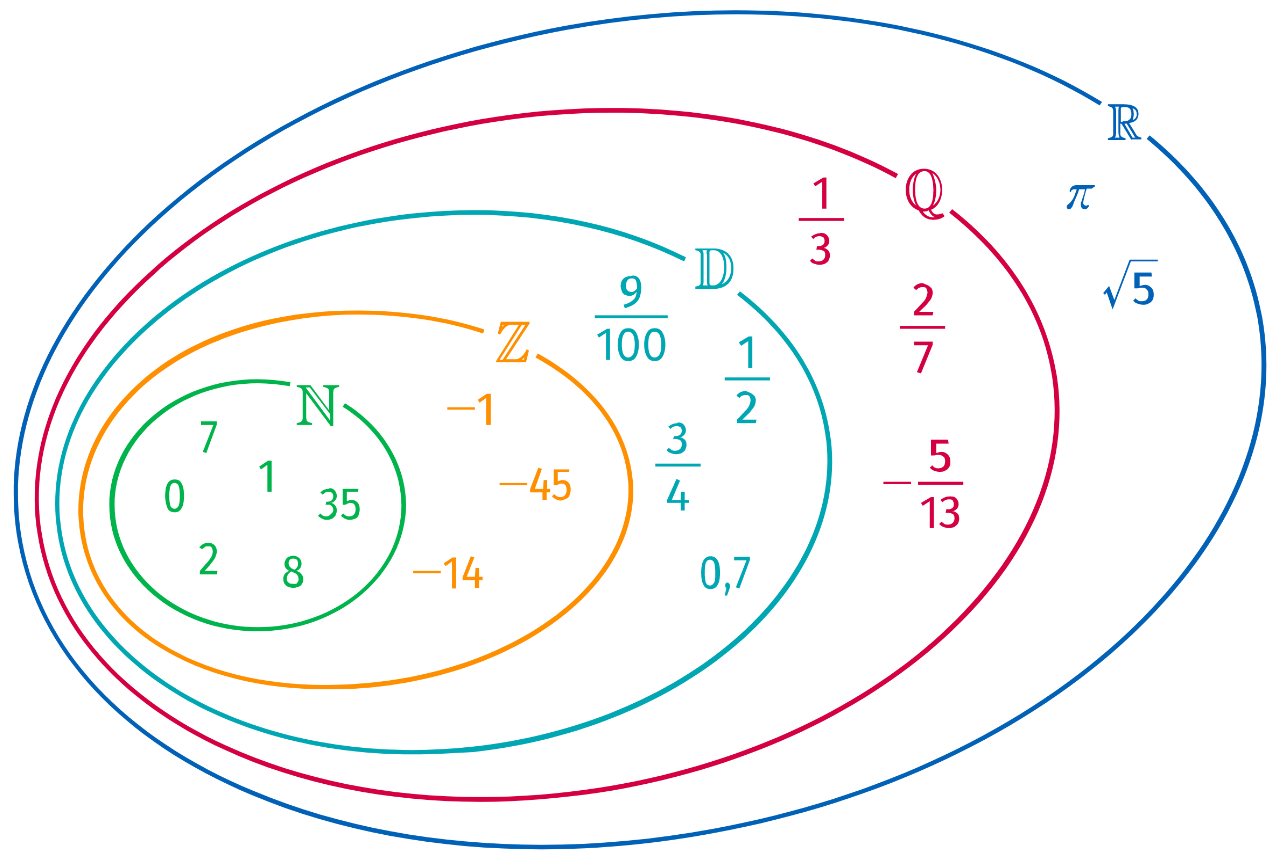
\includegraphics[width=1.0\textwidth]{Ensemble.png}
\caption{Les ensembles de nombres}
\label{fig:Ensembles}
\end{figure}



\section{La droite des réels}

On peut représenter chaque réel$x\in\R$ sur une droite graduée. C'est à dire 
qu'à tout point de la droite graduée on peut associer un réel $x$:

\begin{center}
\definecolor{xdxdff}{rgb}{0.49019607843137253,0.49019607843137253,1.}
\definecolor{uuuuuu}{rgb}{0.26666666666666666,0.26666666666666666,0.26666666666666666}
\begin{tikzpicture}[line cap=round,line join=round,x=1.0cm,y=1.0cm]
\clip(-4.,-1.) rectangle (5.,1.);
\draw [domain=-5.4:6.2] plot(\x,{(-0.-0.*\x)/6.16});
\draw (1.56,-0.02) node[anchor=north west] {$x$};
\begin{scriptsize}
\draw [fill=uuuuuu] (0.,0.) circle (1.5pt);
\draw[color=uuuuuu] (0.14,0.28) node {$O$};
\draw [fill=xdxdff] (1.66,0.) circle (1.5pt);
\draw[color=xdxdff] (1.8,0.28) node {$M$};
\end{scriptsize}
\end{tikzpicture}
\end{center}
On dit que le point $M$ a pour abscisse $x$. Le point $O$ d'abscisse $0$ est appelé origine de la droite.  
\begin{de}[Valeur absolue]
  On appelle valeur absolue d'un réel $x$ la distance entre le point $M$ et 
  l'origine $O$ de la droite des réels. La valeur absolue de $x$ se note $|x|$. 
  C'est un nombre positif ou nul.
\end{de}

Un nombre est donc toujours égal à sa valeur absolue multipliée par $1$ ou $-1$. En fait, un nombre est constitué de deux parties :
\begin{itemize}
    \item Son signe, qui peut être $+$ ou $-$
    \item Sa valeur absolue, qui est donc en quelque sorte la "valeur quantitative" d'un nombre.
\end{itemize}



\begin{exe}
  On considère les points $M$ et $C$ ci-dessous:
  \begin{center}
    \definecolor{xdxdff}{rgb}{0.49019607843137253,0.49019607843137253,1.}
\definecolor{xdxdff}{rgb}{0.49019607843137253,0.49019607843137253,1.}
\definecolor{uuuuuu}{rgb}{0.26666666666666666,0.26666666666666666,0.26666666666666666}
\begin{tikzpicture}[line cap=round,line join=round,x=1.0cm,y=1.0cm]
\clip(-4.,-1.) rectangle (5.,1.);
\draw [domain=-4.:5.] plot(\x,{(-0.-0.*\x)/6.16});
\draw (1.56,-0.02) node[anchor=north west] {$x=1,7$};
\draw (-2.84,-0.18) node[anchor=north west] {$y=-2,6$};
\begin{scriptsize}
\draw [fill=uuuuuu] (0.,0.) circle (1.5pt);
\draw[color=uuuuuu] (0.14,0.28) node {$O$};
\draw [fill=xdxdff] (1.66,0.) circle (1.5pt);
\draw[color=xdxdff] (1.8,0.28) node {$M$};
\draw [fill=xdxdff] (-2.48,0.) circle (1.5pt);
\draw[color=xdxdff] (-2.34,0.28) node {$C$};
\end{scriptsize}
\end{tikzpicture}
  \end{center}
  
  On a alors $|y|=2,6$ et $|x|=1,7$.
\end{exe}

\begin{prop}[Distance entre deux points] On considère le point $A$ d'abscisse $a$ 
  et le point $B$ d'abscisse $b$. La distance $AB$ est la valeur absolue de la 
  différence entre $a$ et $b$. C'est à dire $AB=|b-a|$. 
\end{prop}
  \section{Intervalles de $\R$}
  
  \begin{de}[Symbole de l'infini]
    En mathématiques on note $\infty$ pour dire l'infini.
  \end{de}
  

  \begin{de}[Ordre]
    Soient $x$ et $y$ deux nombre réels on a alors forcément une (et seulement une) des trois situations suivantes :
    \begin{enumerate}
      \item $x$ est égal à $y$. On note classiquement $x=y$.
      \item $x$ est plus petit que $y$. On note $x\leq y$ ou $x<y$ (strictement plus petit). 
      \item $x$ est plus grand que $y$. On note $y\geq x$ ou $y>x$ (strictement plus 
      grand). 
    \end{enumerate}
  \end{de}
  
  \subsection{Les intervalles}
  
  \begin{de}[intervalle]
    Un \underline{intervalle} de $\R$ est l'ensemble des nombres compris entre deux valeurs 
    fixées. Ces deux valeurs peuvent-être infinies. 
  \end{de}
  
  \subsection*{Les huit types d'intervalles}
  Soient $a$ et $b$ deux réels. On donne les différentes définitions sous forme 
  d'équivalences. Le symbole $\Longleftrightarrow$ signifie équivalent. 
  \begin{enumerate}
    \item Les intervalles bornés
    \begin{enumerate}
      \item Intervalle fermé borné $[a;b]$: 
      $$x\in[a;b]\Longleftrightarrow a\leq x\leq b$$
      Ici $x$ peut être égal à $a$ ou à $b$.
      \item Intervalle semi ouvert borné $]a;b]$ ou $[a;b[$: 
      $$x\in]a;b]\Longleftrightarrow a<x\leq b$$
      $$x\in[a;b[\Longleftrightarrow a\leq x< b$$
      Dans un cas $x$ ne peut pas être égal à $a$ et dans l'autre $x$ ne peut 
      pas être égal à $b$. 
       \item Intervalle ouvert borné $]a;b[$: 
      $$x\in]a;b[\Longleftrightarrow a< x< b$$
      Ici $x$ ne peut pas être égal à $a$ et à $b$.
    \end{enumerate}
    \begin{de}
      Les réels $a$ et $b$ s'appellent les bornes de l'intervalle.
    \end{de}
    \item Intervalles non bornés:
    \begin{enumerate}
      \item $$x\in[a;+\infty[\Longleftrightarrow x\geq a$$
      \item $$x\in]-\infty;a]\Longleftrightarrow x\leq a$$
      \item $$x\in]a;+\infty[\Longleftrightarrow x<a$$
      \item $$x\in]-\infty;a[\Longleftrightarrow x> a$$
    \end{enumerate}
  \end{enumerate}
   Remarques : \begin{itemize}
      \item On peut définir $\R$ comme un intervalle :  $]-\infty;+\infty[$
      \item L'infini n'étant pas un nombre réel, un intervalle est toujours ouvert en l'infini (plus ou moins)
  \end{itemize}
  
  
  \subsection*{Réels compris dans un intervalle de longueur donnée}
  On considère un intervalle \textbf{borné} (ouvert ou fermé). 
  \begin{de}
    Soient $a<b$ deux réels. La \underline{longueur} d'un intervalle borné entre $a$ et $b$ 
    est le réel $b-a$. On l'appelle aussi \underline{amplitude} de l'intervalle.
  \end{de}

\section{Les dernières notations du chapitre}

\subsection{Equivalence}

Un \underline{prédicat} est une proposition qui peut être vraie ou fausse, elle peut dépendre d'une variable. 

Exemples :
\begin{itemize}
    \item $1=0$ est un prédicat qui est toujours faux.
    \item $3 = \frac{6}{2}$ est un prédicat qui est toujours vrai.
    \item $x - 1 = 0$ est un prédicat qui sera vrai ou faux selon la valeur de $x$.
\end{itemize}

\begin{de}
    Deux prédicats sont dits équivalents si les situations où ils sont vrais sont les mêmes. On note cette relation $\Leftrightarrow$
\end{de}

Exemples :
\begin{itemize}
    \item On a vu dans le chapitre sur les équations que $x-3 = 0 \Leftrightarrow x = 3$ : les deux prédicats auront le même statut (vrai ou faux) quel que soit x
    \item Dès qu'on a plusieurs manières d'écrire un prédicat, on peut dire que les prédicats sont équivalents. Par exemple pour les intervalles : $x \in [3,5] \Leftrightarrow  3 \leq x \leq 5$
\end{itemize}

\subsection{Union et intersections d'ensembles}

\begin{de}
    Soient deux ensembles $E$ et $F$ :
    \begin{itemize}
        \item $E \cup F$ (on dit "$E$ union $F$") représente l'union de $E$ et de $F$. C'est l'ensemble des éléments qui appartiennent à $E$ \textbf{ou} à $F$
        \item $E \cap F$ (on dit "$E$ inter $F$") représente l'ensemble des éléments qui appartiennent à $E$ \textbf{et} à $F$
        \item $E \setminus F$ (on dit "$E$ privé de $F$) représente l'ensemble des éléments qui appartiennent à $E$ \textbf{mais pas} à $F$
    \end{itemize}
\end{de}



Exemple : \begin{itemize}
    \item Soient $E = \{1;2;4;8\}$ et $F = \{2;4;6;8\}$. $E \cup F = \{1;2;4;6;8\}$ et $E \cap F = \{2;4;8\}$
    \item Mettre une étoile $*$ à côté d'un ensemble comme $\N$ ou $\R$, c'est lui enlever l'élément $0$ :  $\R^* = \R \setminus \{0\}$
\end{itemize}

    

\begin{figure}
    \centering
    \begin{minipage}{0.3\textwidth}
        \centering
        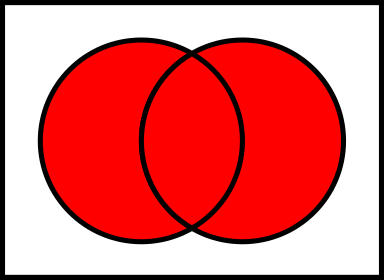
\includegraphics[width=0.9\textwidth]{Venn0111.png} 
        \caption{Union :  $E \cup F$}
    \end{minipage}
    \begin{minipage}{0.3\textwidth}
        \centering
        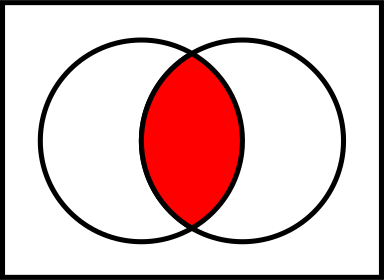
\includegraphics[width=0.9\textwidth]{Venn0001.png} 
        \caption{Intersection :  $E \cap F$}
    \end{minipage}
    \begin{minipage}{0.3\textwidth}
        \centering
        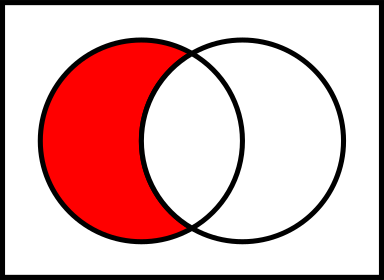
\includegraphics[width=0.9\textwidth]{Venn0100.png}
        \caption{Différence : $E \setminus F$}
    \end{minipage}
\end{figure}
   
 
\begin{figure}
 \begin{tabular}{|c|p{0.3\linewidth}|p{0.5\linewidth}|}
    \hline
    Notation & Comment le lire & Comment l'utiliser  \\\hline
    $\emptyset$ & "Ensemble vide" & Désigne l'ensemble qui ne contient aucun élément (il est unique!) \\ \hline
    $\in, \notin$ & "Appartient à" / "N'appartient pas à" & Signale que l'élément à gauche du signe appartient (ou non) à l'ensemble à droite du signe. \\ \hline
    $\subset, \not\subset$ & "Est inclus dans" / "N'est pas inclus dans" & Signale que l'ensemble de gauche est inclus dans l'ensemble de droite. \\ \hline
    $\N, \Z, \D, \Q, \R$ & "Grand N" (etc...) & Désigne l'ensemble de nombre correspondant dans le cours : entiers naturels, entiers relatifs, décimaux, rationnels et réels \\ \hline
    $\left[2,3\right]$ & "L'intervalle 2, 3 fermé" & Tous les nombres contenus entre le nombre de gauche de l'intervalle et le nombre de droite, bornes incluses\\ \hline
    $\left]2,3\right[$ & "L'intervalle 2, 3 ouvert" & Tous les nombres contenus entre le nombre de gauche de l'intervalle et le nombre de droite, bornes non incluses\\ \hline
    $\lvert x \rvert$ & "Valeur absolue de $x$" & Désigne la valeur absolue d'un nombre (c'est à dire sa valeur numérique à laquelle on a retiré le signe s'il est négatif). \\ \hline
    $\infty, + \infty$ & "L'infini", "plus l'infini" & Désigne le concept d'infini : une grandeur plus grande que n'importe quel nombre réel. \\ \hline
    $A \cup B$ & "A union B" & Pour noter tous les éléments contenus dans \textbf{n'importe quel} ensemble à gauche ou à droite du signe \\ \hline
    $A \cap B$ & "A inter B" & Pour noter tous les éléments contenus dans \textbf{les deux} ensembles décrits à gauche et à droite du signe. \\ \hline
    $A \setminus B$ & "A privé de B" & Pour noter tous les éléments contenus dans l'ensemble de gauche mais pas l'ensemble de droite. \\ \hline
    
    $\Leftrightarrow$ & "est équivalent à" & Signale que la proposition de droite est équivalente à la proposition de gauche : L'une est vraie si et seulement si l'autre est vraie \\ \hline
    $\{1;2;4\}$ & "L'ensemble contenant les nombres 1, 2 et 4" & Désigne l'ensemble constitué des éléments situés entre les $\{\}$\\ \hline 
    $\R^*$ & "Grand R étoile" & Signale qu'on a retiré le nombre 0 de l'ensemble de nombre à gauche. Ici, on a tous les réels non nuls \\ \hline
    $\R^+$ & "Grand R +" & Signale qu'on considère seulement les nombres positifs de l'ensemble à gauche du "+". Ici on désigne tous les réels positifs ou nuls.\\ \hline

 \end{tabular}
\caption{Les (nombreuses) notations vues dans le chapitre}
\label{fig:Notations}
\end{figure}


\chapter{Fonctions : généralités}

\section{Définition}

Les objets mathématiques ont chacun un rôle. Le rôle d'une fonction est d'\textbf{associer}. Associer, cela veut dire transformer un objet en un autre. Cette année, on verra surtout les fonctions qui transforment un nombre réel en un autre nombre réel, mais une fonction peut techniquement associer n'importe quel type d'objet à n'importe quel autre :
\begin{itemize}
    \item Fonction qui associe à une chaîne de caractère son initiale
    \item Fonction qui associe un point à un autre. Par exemple, on peut associer chaque point qui se trouve sur une carte de la ville au point auquel il correspond dans la vraie vie. Plus mathématiquement, une symétrie est un point qui va associer à chaque point un autre.
\end{itemize}

Dans le cours de mathématiques, on utilisera presque exclusivement des fonctions d'un intervalle réel dans les nombres réels.  Il est à noter qu'en python, on utilisera des fonctions dans un sens plus large.

\begin{de}[Fonction d'un intervalle de $\R$]
    Soit $I$ un intervalle de $\R$. On dit que $f$ est une \underline{fonction} de $I$ dans $\R$ si à tout élément $x$ de $I$,  $f$ associe un et un seul élément de $\R$, qu'on note $f(x)$.
    On note :
        \[
        \begin{array}{ccccc}
        f & : & I & \to & \R \\
         & & x & \mapsto & f(x) \\
        \end{array}
        \]
\end{de}

$x$ est appelée la \underline{variable} de la fonction $f$. On l'appelle variable tant qu'on ne lui fixe pas de valeur. Ce terme sera seulement utilisé pour : \begin{itemize}
    \item Dire que $x$ n'a pas encore été fixé et qu'il peut donc varier
    \item Décrire le nombre de variables d'une fonction.
\end{itemize}

Dans l'année, on étudiera beaucoup de fonctions à une variable, mais il y a aussi des fonctions à deux variables (ou encore plus), et vous avez même probablement vu des fonctions à deux variables avant les fonctions à une variable : l'addition par exemple, est une fonction qui prend deux nombres en entrée, et qui ressort un nombre en sortie. On pourrait aussi bien déclarer que l'addition est une fonction à deux variables, qui prend en entrée deux nombres réels, et qui leur associe un nombre réel : leur somme.



Exemple :  la fonction carré : à tout nombre réel $x$, elle associe $x^2$. Si on appelle g cette fonction, on note :
\[
\begin{array}{ccccc}
f & : & \R & \to & \R \\
 & & x & \mapsto & x^2 \\
\end{array}
\]


\subsection{Image et antécédent, tableau de valeurs}

\begin{de}
        $f(x)$ s'appelle l' \underline{image} de $x$. On dit que $x$ est \underline{un antécédent} de $f(x)$.
\end{de}

La manière de présenter la fonction qui apparaît ci-dessus est une des manières standard de le faire quand il existe une formule. (On peut aussi noter un peu abusivement La fonction $f$ telle que $f(x)=x^2$ pour tout $x\in \R$.

Mais il n'existe pas toujours de formule simple pour décrire la valeur que prend une fonction selon la valeur prise par sa variable. Une manière de la présenter dans ces cas là est de faire appel à un tableau de valeurs.

\begin{de}
    Un tableau de valeurs d'une fonction $f$ est un tableau dans lequel apparaît sur une ligne certaines valeurs prises par la variable, et sur la ligne du dessous l'image de chacune de ces valeurs par la fonction.
\end{de}

Pour la fonction carré, présentée ci-dessus, un tableau de valeur se présenterait ainsi :

\begin{center}
    \begin{tabular}{|c|c|c|c|c|c|c|}
    \hline
         $x$ & $-1$ & $0$ & $1$ & $2$&$3$ & $4$ \\
    \hline
         $f(x)$ & $1$ & $0$ &$1$&$4$&$9$&$16$ \\
    \hline
    \end{tabular}
\end{center}

\section{Représentation graphique}

Avant de pouvoir tracer la courbe représentative d'une fonction, il nous faut savoir associer à des coordonnées un point du plan, et vice-versa. Pour cela, on utilise un repère.

\begin{de}[Repère]
Pour repérer un point dans le plan, on trace deux droites (les axes) sécants en un point $O$, origine du repère. Sur un axe, on place un point $I$ et la distance $OI$ sert de référence. De même sur l'autre axe on place un point $J$ et la distance $OJ$ sert de référence. $(O;I,J)$ défini un repère du plan. 

 Soit $M$ un point quelconque. On trace les parallèles aux axes passant par $M$. Elles coupent ces deux axes en $M'$ et $M"$.

$M'$ est repéré par un nombre $x_{M}$ sur l'axe $[OI)$ et $M"$ par un nombre $y_{M}$ sur l'axe $[OJ)$.

On dit que $x_{M}$ et $y_{M}$ sont les coordonnées de M dans le repère $(O;I;J)$. $x_{M}$ est l’abscisse de $M$ et $y_{M}$ l’ordonnée de $M$.
\end{de}


On représente en règle générale les fonctions dans un repère orthonormé, c'est à dire que les droites $(OI)$ et $(OJ)$ seront perpendiculaires, et que les longueurs $OI$ et $OJ$ seront égales.

\begin{center}
    \begin{tabular}{|c|c|c|}
        \hline
         Axe & Nom & Lettre associée  \\
        \hline
        Horizontal & Abscisse & x \\
        \hline
        Vertical & Ordonnées & y \\
        \hline
    \end{tabular}
\end{center}

\begin{de}[Courbe représentative d'une fonction]
    La courbe représentative d'une fonction $f$ est l'ensemble des points $(x,f(x))$, où $x$ parcourt l'ensemble des points où la fonction est définie, qu'on a placé sur un repère orthonormé.
\end{de}

\begin{minipage}{0.6\textwidth}
    Concrètement, pour représenter une fonction, on commence par faire un tableau de valeurs pour calculer l'image de certains points qui seront situés dans la partie de l'axe des abscisses que l'on représente. Puis on place ces points sur le repère. Enfin, on relie ces points par une courbe, dont l'allure dépend de la manière dont la fonction est définie (Elle ne va pas en ligne droite entre les points du tableau de valeur, sauf si la fonction est affine sur l'intervalle entre les deux points). Pour cette dernière partie, on peut s'aider de la représentation graphique sur une calculatrice, de son expérience, ou rajouter des valeurs supplémentaires dans le tableau de valeur pour voir ce que la courbe fait entre les points qu'on a tracé.
    \begin{enumerate}
        \item Tracer un repère
        \item Préparer un tableau de valeurs de la fonction
        \item Placer les points du tableau de valeur sur le repère
        \item Tracer une courbe qui passe par ces points
    \end{enumerate}
\end{minipage}

\begin{minipage}{0.35\textwidth}
  \begin{tikzpicture}
   \begin{axis}[
	 name = graph1,
     ytick distance = 1,
     xtick distance = 1,
     ymin=-1.1, ymax=9.1,
     xmin=-4.1, xmax=4.1,
     grid=both,
     grid style={line width=.1pt,draw=brown!20},
     major grid style={line width=.2pt,draw=brown!40},
     minor tick num=9,
     tick style={draw=none},
   ]

     \addplot [domain=-10:10, samples=500, color=gray!90]
        {x^2};
    \addplot[domain=-10:10,samples=21,only marks, mark=x, blue] {x^2}; 
   \end{axis}
   \node[anchor=north] at (graph1.south) {\scriptsize Courbe représentative de $f(x)= x^ 2$  };
  \end{tikzpicture}
\end{minipage}

\section{Fonctions et équations}

Soit $f$ une fonction définie sur un sous-ensemble des réels, et $a$ un nombre.

\begin{minipage}{0.5\textwidth}  
Résoudre $f(x)=a$ c'est trouver tous les antécédents de $a$ par la fonction $f$.  
\newline ~ \newline
Graphiquement, c'est trouver toutes les abscisses en lesquelles la courbe représentative de la fonction croise la droite horizontale d'ordonnée $a$.
\end{minipage}
\begin{minipage}{0.35\textwidth}
  \begin{tikzpicture}
   \begin{axis}[
	 name = graph1,
     ytick distance = 1,
     xtick distance = 1,
     ymin=-1.1, ymax=6.1,
     xmin=-3.1, xmax=3.1,
     grid=both,
     grid style={line width=.1pt,draw=brown!20},
     major grid style={line width=.2pt,draw=brown!40},
     minor tick num=9,
     tick style={draw=none},
   ]
     \addplot [domain=-10:10, samples=500, color=gray!90]
        {x^2};
     \addplot [domain=-10:10, samples=500, color=blue]
        {3};
     \addplot[only marks, mark=x]coordinates{ (1.73205,3)
		(-1.73205,3)};
      \draw [thick,dashed] (1.73205,0) -- (1.73205,3);
      \draw [thick,dashed] (-1.73205,0) -- (-1.73205,3);
   \end{axis}
   \node[anchor=north][text width=\textwidth][align=center] at (graph1.south) {\scriptsize Résolution graphique de $x^2=3$ :  les deux solutions valent environ $-1.7$ et $1.7$ };
  \end{tikzpicture}
\end{minipage}

On peut appliquer cela à toutes les équations : Les équations à une inconnue, qu'on notera ici $x$, sont toujours de la forme $A(x)=B(x)$ où A et B sont des fonctions, puisque les deux membres de l'égalité sont calculables pour un $x$ donné.
On peut donc toujours la transformer en une égalité de la forme $f(x)=0$, où $f(x)=A(x)-B(x)$  ($f$ est la différence de deux fonctions, c'est donc elle même une fonction)


\subsection{Inéquation}

\begin{de}
    Une \underline{inéquation}, c'est une inégalité entre deux expressions qui s'expriment chacune en fonction d'une même inconnue. Comme dans le cadre d'une équation, \underline{résoudre une inéquation} c'est trouver toutes les valeurs de l'inconnue qui rendent l'inégalité vraie.
\end{de}



\begin{minipage}{0.5\textwidth}  
Résoudre $f(x) \geq a$ c'est trouver tous les antécédents de nombres plus petits que $a$ par la fonction $f$.
\newline ~ \newline
Graphiquement, c'est trouver toutes les abscisses en lesquelles la courbe représentative de la fonction est \textbf{en dessous} de l'ordonnée $a$ (c'est à dire en dessous de la droite d'équation $y=a$.
\newline ~ \newline
A l'inverse, Résoudre $f(x) \geq a$ c'est trouver tous les antécédents de nombres plus grands que $a$ par la fonction $f$.
Graphiquement, c'est trouver toutes les abscisses en lesquelles la courbe représentative de la fonction est \textbf{au dessus} de la droite d'équation $y=a$.
\end{minipage}

\begin{minipage}{0.35\textwidth}
  \begin{tikzpicture}
   \begin{axis}[
	 name = graph1,
     ytick distance = 1,
     xtick distance = 1,
     ymin=-1.1, ymax=2.1,
     xmin=-3.1, xmax=3.1,
     grid=both,
     grid style={line width=.1pt,draw=brown!20},
     major grid style={line width=.2pt,draw=brown!40},
     minor tick num=9,
     tick style={draw=none},
   ]
     \addplot [domain=-10:10, samples=500, color=gray!90]
        {x^2};
     \addplot [domain=-10:10, samples=500, color=blue]
        {1};
     \addplot[only marks, mark=x]coordinates{ (1,1)
		(-1,1)};
      \draw [thick,dashed] (1,0) -- (1,1);
      \draw [thick,dashed] (-1,0) -- (-1,1);
      \draw[red, line width = 3pt] (-1,0) --(1,0); 
        \node[red, line width = 3pt] at (-1,0) {$\Big[$};
        \node[red, line width = 3pt] at (1,0) {$\Big]$};
   \end{axis}
   \node[anchor=north][text width=\textwidth][align=center] at (graph1.south) {\scriptsize Résolution graphique de $x^2 \leq 1$ :  Les solutions valides sont les $x$ de $[-1;1]$ };
\end{tikzpicture}  \begin{tikzpicture}
   \begin{axis}[
	 name = graph1,
     ytick distance = 1,
     xtick distance = 1,
     ymin=-1.1, ymax=2.1,
     xmin=-3.1, xmax=3.1,
     grid=both,
     grid style={line width=.1pt,draw=brown!20},
     major grid style={line width=.2pt,draw=brown!40},
     minor tick num=9,
     tick style={draw=none},
   ]
     \addplot [domain=-10:10, samples=500, color=gray!90]
        {x^2};
     \addplot [domain=-10:10, samples=500, color=blue]
        {1};
     \addplot[only marks, mark=x]coordinates{ (1,1)
		(-1,1)};
      \draw [thick,dashed] (1,0) -- (1,1);
      \draw [thick,dashed] (-1,0) -- (-1,1);
      \draw[red, line width = 3pt] (-3.1,0) --(-1,0);
      \draw[red, line width = 3pt] (1,0) --(3.1,0); 
        \node[red, line width = 3pt] at (-1,0) {$\Big]$};
        \node[red, line width = 3pt] at (1,0) {$\Big[$};
   \end{axis}
   \node[anchor=north][text width=\textwidth][align=center] at (graph1.south) {\scriptsize Les solutions valides de $x^2 \geq 1$ sont les $x$ de $]-\infty;1] \cup [1;+\infty[$ };
  \end{tikzpicture}
\end{minipage}

\section{Parité d'une fonction}

Ces propriétés permettent notamment de tracer le graphique d'une fonction sur les entiers négatifs, elles divisent donc la quantité de travail par 2.

\begin{de}
    Une fonction $f$ est dite paire si l'image de l'opposé de tout nombre de son ensemble de définition est égale à l'image de ce nombre. Pour tout nombre $x$ tel que $f(x)$ est défini  alors $f(-x)$ est défini et 
    \vspace{0.3cm}
    \begin{center}
    $f(x)=f(-x)$
    \end{center}
\end{de}

Graphiquement, la courbe représentative d'une fonction paire sera symétrique par rapport à l'axe des ordonnées dans un repère orthonormé. (Donc par rapport à  \textbf{une droite})

Par exemple, la fonction carré est paire : pour tout $x$ réel, $x^2=(-x)^2$


\begin{de}
    Une fonction $f$ est dite impaire si l'image de l'opposé de tout nombre de son ensemble de définition est égale à l'opposé de l'image de ce nombre. Pour tout nombre $x$ tel que $f(x)$ est défini  alors $f(-x)$ est défini et 
    \vspace{0.3cm}
    \begin{center}
    $f(-x)=-f(x)$
    \end{center}
\end{de}

Graphiquement, la courbe représentative d'une fonction impaire sera symétrique par rapport à l'origine dans un repère orthonormé (Donc par rapport à  \textbf{un point})

Par exemple, la fonction inverse, qui à tout $x$ non nul associe $\frac{1}{x}$  est impaire : pour tout $x$ réel, $x^2=(-x)^2$
\begin{center}
  \begin{tikzpicture}
   \begin{axis}[
	 name = graph1,
     ytick distance = 1,
     xtick distance = 1,
     ymin=-3.1, ymax=3.1,
     xmin=-3.1, xmax=3.1,
     grid=both,
     grid style={line width=.1pt,draw=brown!20},
     major grid style={line width=.2pt,draw=brown!40},
     minor tick num=9,
     tick style={draw=none},
   ]

     \addplot [domain=-10:10, samples=500, color=gray!90]
        {1/x};
   \end{axis}
   \node[anchor=north] at (graph1.south) {\scriptsize La Courbe représentative de $g(x)= \frac{1}{x}$ est impaire  };
  \end{tikzpicture}
\end{center}

\section{Sens de variation d'une fonction}

\begin{de}
    Une fonction $f$ est dite \underline{croissante} sur un intervalle $I$ si pour deux nombres $a$ et $b$ de cet intervalle :
    \vspace{0.3cm}
    \begin{center}
    si $a \leq b$,  alors $f(a) \leq f(b)$
    \end{center}
\end{de}

Remarques :
\begin{itemize}
    \item On dit souvent qu'une fonction croissante sur un intervalle conserve l'ordre : Comparer (au sens de "se demander quel nombre est le plus grand") les images de deux éléments donnera le même résultat que comparer ces deux éléments.
    \item Graphiquement, la courbe représentative sur un intervalle "montera" : en parcourant la courbe de gauche à droite, l'image en ordonnée devient de plus en plus haute.
\end{itemize}

Une fonction décroissante, c'est le contraire :

\begin{de}
    Une fonction est dite \underline{décroissante} sur un intervalle $I$ si pour deux nombres $a$ et $b$ de cet intervalle :
    \vspace{0.3cm}
    \begin{center}
    si $a \leq b$,  alors $f(a) \geq f(b)$
    \end{center}
\end{de}

\begin{itemize}
    \item On dit souvent qu'une fonction décroissante sur un intervalle inverse l'ordre : Comparer les images de deux éléments donnera le résultat inverse que comparer ces deux éléments.
    \item Graphiquement, la courbe représentative sur un intervalle "descend" : en parcourant la courbe de gauche à droite, l'image en ordonnée devient de plus en plus basse.
    \item Sur un intervalle donné, une fonction qui est soit décroissante, soit croissante est dite \underline{monotone}. Attention, la fonction doit garder le même sens de variation tout au long de l'intervalle.
\end{itemize}

Contrairement aux fonctions affines que vous aviez vu jusqu'à présent, qui gardaient toujours le même sens de variation, une fonction peut être croissante sur certains intervalles et décroissante sur d'autres. 

La fonction carré est croissante sur $\R^+=[0;+\infty[$ c'est à dire sur les réels positifs et décroissante sur $]-\infty;0]$.  En revanche, on ne peut pas dire qu'elle est monotone sur $\R$, car elle ne reste pas monotone sur l'intervalle.

\section{Tableau de variations d'une fonction}

Un \underline{tableau de variations} résume en un seul schéma des informations importantes sur une fonction.

\begin{minipage}{0.7\textwidth}
    Ainsi, le tableau ci-dessous présente les variations de la fonction $f$ définie sur l'intervalle $[-3;3]$ par $f(x)=2x^3+3x^2-12x$, dont la courbe représentative apparaît à droite.
    \newline
    
    \vspace{1 cm}
    Tableau de variations de la fonction $f$ : \newline
    
    \begin{tikzpicture}
       \tkzTabInit{$x$ / 1 , $f(x)$ / 2}{$-3$, $-2$, $1$, $3$}
       \tkzTabVar{-/ $9$, +/ $20$, -/ $-7$ , +/ $45$ }
    \end{tikzpicture}
\end{minipage}

\begin{minipage}{0.25\textwidth}
    \centering
    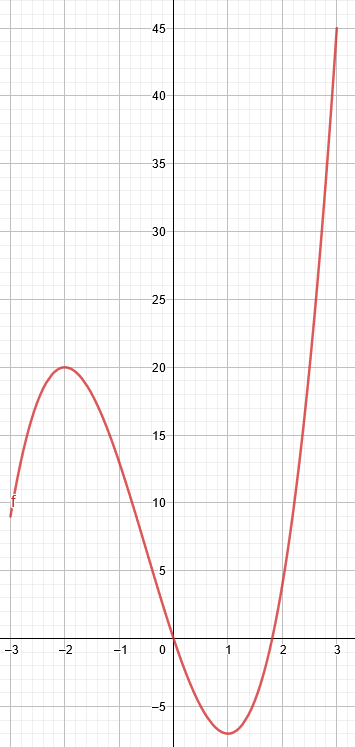
\includegraphics[width=0.9\textwidth]{20221101_CourbeRepTabloVariation.PNG} 
\end{minipage}

Sur la première ligne d'un tableau de variations d'une fonction figurent les antécédents remarquables par la fonction $f$ :\begin{itemize}
    \item Les bornes de l'intervalle où la fonction est définie
    \item Les bornes des intervalles où la fonction est monotone (Ce sont les points où la fonction change de sens de variation)
\end{itemize}

La deuxième partie d'un tableau de variations indique les intervalles croissants par une flèche qui va vers le haut, et les intervalles décroissants par une flèche qui va vers le bas. Puis, on écrit sous les valeurs de la première ligne leurs images par la fonction.

\subsection{Extremums d'une fonction}

Un extremum est une valeur extrême, prise par une fonction sur un intervalle donné. Cela peut être un minimum ou un maximum.

\begin{de}
    On dit que $f$ admet un \underline{maximum} sur l'intervalle $I$ en la valeur $a \in I$ si pour tout $x \in I,  f(x)\leq f(a)$.
    On dit que $f$ admet un \underline{minimum} sur l'intervalle $I$ en la valeur $a \in I$ si pour tout $x \in I, f(x) \geq f(a)$. 
\end{de}

Si l'intervalle $I$ est l'ensemble sur lequel la fonction est défini, on parle de maximum (ou minimum) \textbf{global}. Sinon, on parle de maximum (ou minimum) \textbf{local}.

Les valeurs au bord des intervalles fermés qui apparaissent dans des tableaux de variation sont des extremums locaux.

Par exemple, dans le tableau ci-dessus\begin{itemize}
    \item 
$f(-2)=20$ est la valeur maximum prise par la fonction sur l'intervalle $[-3;1]$. $f$ admet un maximum local en $-2$ qui vaut $20$. 
\item $f$ admet un minimum global en $1$, en lequel elle prend la valeur de $-7$.
\end{itemize} 

\chapter{Vecteurs du plan}

Dans un repère, on place deux points $A$ et $B$. Intuitivement, un vecteur décrit le chemin à parcourir pour passer de $A$ à $B$. C'est un déplacement, qu'on appelle translation.

\begin{de}[Translation]
  Rappel : Une \underline{translation} est une glissade qui transforme un point du plan en un autre. Opérer une translation sur une figure, c'est effectuer \textbf{la même} translation à tous les points de la figure.
  Opérer une translation sur une figure conserve ses distances, ses angles, son aire, et en général toutes les grandeurs qui ne dépendent que du placement des points de la figure les uns par rapport aux autres. 
\end{de}

\begin{de}[Vecteur]
La translation qui transforme le point $A$ en le point $B$. est appelée translation de \underline{vecteur} $\overrightarrow{AB}$.
\end{de}

On peut noter un vecteur par son point de départ et son point d'arrivée. On peut également lui donner son propre nom, qui est souvent $\overrightarrow{u}$ ou $\overrightarrow{v}$ (ici, $u$ et $v$ sont en minuscule, car on réserve généralement les lettres majuscules  pour les points du plan).

\begin{center}
  \begin{tikzpicture}
    \draw[->](0,0)node[left]{A}--(2,1)node[right]{B};
  \end{tikzpicture}
\end{center}

On va commencer par décrire les vecteurs dans le plan muni d'un repère cartésien. Cela facilite les notations. Puis nous verrons les propriétés dans un cadre plus général.

\section{Dans un repère cartésien.}

\subsection{Coordonnées d'un vecteur}

Un vecteur représente un chemin d'un point à un autre du plan En deux dimensions. Si l'on dispose d'un repère cartésien, on peut décrire un vecteur par deux coordonnée : Le déplacement effectué sur l'axe des abscisses, et le déplacement effectué sur l'axe des ordonnées.



\newcommand*{\Coord}[2]{% 
  \ensuremath{ 
    \begin{pmatrix} 
      #1\\ 
      #2 
    \end{pmatrix}}}

\begin{minipage}{0.25\textwidth}
    
Pour passer du point $A(1,3)$ au point $B(5,4)$, on se déplace de $+4$ sur l'axe des abscisses et de $+1$ sur l'axe des ordonnées.

Le vecteur $\overrightarrow{u}=\overrightarrow{AB}$ a donc pour coordonnées $\Coord{4}{1}$.

On peut également le noter $\overrightarrow{AB}\Coord{4}{1}$

On peut voir un vecteur comme un plan de route : Pour atteindre $B$ en partant de $A$, avancez de $4$ sur l'axe des abscisses, et de $1$ sur l'axe des ordonnées.

\end{minipage}
\begin{minipage}{0.7\textwidth}
    \centering
    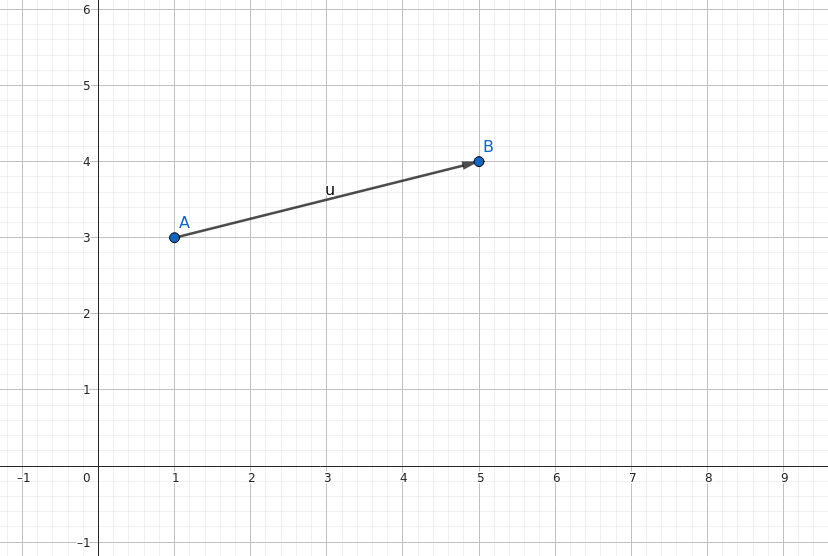
\includegraphics[width=0.9\textwidth]{vecteurExemple.png} 
\end{minipage}

On note les coordonnées d'un vecteur verticalement. Si la translation diminue les abscisses ou les ordonnées, la coordonnée du vecteur associé sera négative.

\begin{prop}
    Soient deux points $M(x_M,y_M)$ et $M'(x_{M'},y_{M'})$ dans un repère. Les coordonnées du vecteur $\overrightarrow{MM'}$ sont $\Coord{x_{M'}-x_{M}}{y_{M'}-y_{M}}$.
\end{prop}

Note : C'est simplement la formule de la différence de deux points en deux dimensions.


\begin{de}
    Deux vecteurs sont égaux s'ils ont les mêmes coordonnées. Attention : On peut dessiner deux fois le même vecteur à différents endroits du plan, et ils seront tout de même égaux.
\end{de}

Quand on dessine sur le plan un vecteur $\overrightarrow{AB}$, égal à un certain vecteur $\overrightarrow{u}$, on dit que $\overrightarrow{AB}$ est un représentant de $\overrightarrow{u}$.

On vous demandera souvent de donner l'image d'un point $C$ par une translation correspondant à un vecteur donné $\overrightarrow{u}$. Pour ce faire, il suffit de donner le point d'arrivée du même vecteur que $\overrightarrow{u}$ partant de $C$.


\begin{minipage}{0.5\textwidth}

La formule est donnée par :

soit $\overrightarrow{u} \Coord{x_u}{y_u}$ un vecteur, et $C(x_c,y_c)$ un point. L'image $C'$ de $C$ par la translation de vecteur $u$ a pour coordonnées $C'(x_c+x_u, y_c+ y_u)$.

\end{minipage}
\begin{minipage}{0.45\textwidth}
  Cela correspond au dessin :
    \centering
    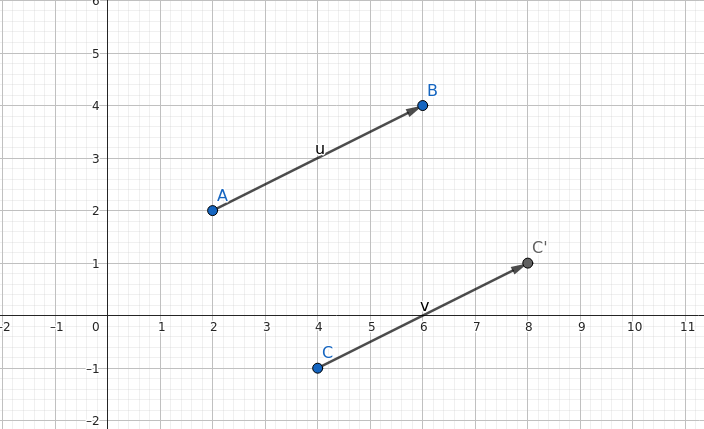
\includegraphics[width=0.9\textwidth]{Vecteurs_C+u.png} 

\end{minipage}



\subsection{vecteur nul}

\begin{de}
    Le vecteur nul est le vecteur de coordonnées $\Coord{0}{0}$. Il est le vecteur associé à la translation qui transforme tout point en lui-même. On le note $\overrightarrow{0}$
\end{de}

Note : En général, on ne dessine pas le vecteur nul.

\subsection{Somme de vecteurs}

Effectuer plusieurs translations d'affilée revient à effectuer une seule translation, associée à un vecteur qui correspond à la somme des vecteurs directeurs des translations : $\overrightarrow{u}+\overrightarrow{v}$ aura pour coordonnées la somme termes à termes des coordonnées de $\overrightarrow{u}$ et de $\overrightarrow{v}$.

\begin{de}
    Soient $\overrightarrow{u} \Coord{x_{\overrightarrow{u}}}{y_{\overrightarrow{u}}}$ et 
    $\overrightarrow{v} \Coord{x_{\overrightarrow{v}}}{y_{\overrightarrow{v}}}$ deux vecteurs du plan. 
    On note $\overrightarrow{u}+\overrightarrow{v}$ le vecteur de coordonnées 
    $\Coord{x_{\overrightarrow{u}}+x_{\overrightarrow{v}}}{y_{\overrightarrow{u}}+y_{\overrightarrow{v}}}$
\end{de}

\begin{exo}
  Comme l'addition de nombres, l'addition de vecteur est commutative (c'est à dire que $\overrightarrow{u}+\overrightarrow{v} = \overrightarrow{v}+\overrightarrow{u}$) et associative. Le montrer.
\end{exo}

On va voir tout de suite une expression mathématique du fait que vous connaissez sûrement déjà : Aller de Monaco à Paris puis de Paris à Madrid, c'est aller de Monaco à Madrid.

\begin{prop}[Relation de Chasles]
  Soient $A$, $B$ et $C$ trois points du plan. 
  \[ \overrightarrow{AB} + \overrightarrow{BC} = \overrightarrow{AC}\]
\end{prop}

Démonstration en exercice (Avec des coordonnées)

\subsection{Multiplication par un nombre réel}

En plus d'additionner deux vecteurs, on peut également les multiplier par un nombre réel. Multiplier un vecteur par le réel $k$, c'est simplement obtenir un chemin $k$ fois plus grand, coordonnée par coordonnée :

\begin{de}
  Soient $\overrightarrow{u} \Coord{x}{y}$ un vecteur du plan, et $k$ un nombre réel. On appelle $k \overrightarrow{u}$, ou $k \times \overrightarrow{u}$, ou $k \cdot \overrightarrow{u}$ le vecteur de coordonnées $\Coord{kx}{ky}$  
\end{de}

\begin{prop}
  Cette multiplication de vecteurs par des réels se comporte comme une multiplication traditionnelle: pour $k$ et $k'$ des nombres réels et $\overrightarrow{u}$ et $\overrightarrow{v}$ deux vecteurs : 
  \begin{enumerate}
    \item $1 \times \overrightarrow{u} = \overrightarrow{u}$, $\overrightarrow{u} + \overrightarrow{u} = 2 \overrightarrow{u}$, $0 \cdot \overrightarrow{u}= \overrightarrow{0}$
    \item $k(\overrightarrow{u} + \overrightarrow{v}) = k\overrightarrow{u} + k\overrightarrow{v}$(distributivité par rapport à l'addition)
    \item $(kk')\overrightarrow{u} = k(k'\overrightarrow{u})$ (Associativité mixte)
  \end{enumerate}
\end{prop}

\subsection{Vecteurs colinéaires}

La colinéarité est une relation, c'est à dire qu'elle n'a un sens quand on parle de deux vecteurs (ou plus). Elle désigne des vecteurs qui pointent dans la même direction (ou dans un direction opposée).
On va cependant voir une définition qui utilise le concept de multiplication par un réel.


\begin{de}[Colinéarité de deux vecteurs]
  Deux vecteurs non nuls $\overrightarrow{u}$ et $\overrightarrow{v}$ sont dits \underline{colinéaires} si $\overrightarrow{u}$ est égal à $\overrightarrow{v}$ multiplié par un certain réel $k$. 
\end{de}

Ainsi, les vecteurs $\overrightarrow{a} \Coord{2}{1}$ et $\overrightarrow{b} \Coord{4}{2}$ sont colinéaires, car $\vec{b}=2\vec{a}$

\begin{prop}
  Deux vecteurs non nuls $\overrightarrow{u} \Coord{x}{y}$ et $\overrightarrow{v} \Coord{x'}{y'}$ sont colinéaires si et seulement si le tableau de leurs coordonnées est un tableau de proportionnalité.
\end{prop}

Toujours avec les mêmes vecteurs $\overrightarrow{a}$ et $\overrightarrow{b}$ qu'à l'exemple précédent,
\begin{tabular}{|c|c|}
  \hline 2 & 4 \\
  \hline 1 & 2\\
  \hline
\end{tabular}  est bien un tableau de proportionnalité.


Remarques : 
\begin{itemize}
  \item la définition ci-dessus ne traite que des vecteurs non nuls. Si l'un des deux vecteurs $u$ et $v$ est nul, alors les deux vecteurs sont forcément colinéaires. Mais ça n'est pas très intéressant, c'est comme de dire que $0$ est un multiple de tous les nombres entiers $n$ puisque $0=0 \times n$.
  \item Cas particulier : Multiplier un vecteur $\overrightarrow{u}$ par $-1$ donne un vecteur dont chaque coordonnée 
  est l'opposé de la coordonnée du vecteur de départ. On appelle le résultat \underline{vecteur opposé} de $\overrightarrow{u}$. On le note $-\overrightarrow{u}$.
  \item Deux vecteurs colinéaires sont les supports de droites parallèles. Cela "se voit" sur un dessin, nous l'énoncerons formellement dans la prochaine partie, et nous clarifierons plus tard dans l'année quand on énoncera plus précisément ce qu'est une droite. 
\end{itemize}

\begin{prop}
  l'opposé d'un vecteur $\overrightarrow{AB}$ est le vecteur $\overrightarrow{BA}$ : Prendre l'opposé d'un vecteur est la même chose que d'inverser le point de départ et d'arrivée. 
\end{prop}

Démonstration : Par la relation de Chasles, $\overrightarrow{AB} + \overrightarrow{BA} = \overrightarrow{AA} = \overrightarrow{0}$. On a donc $\overrightarrow{AB} = \overrightarrow{AB} + \overrightarrow{BA} - \overrightarrow{BA} = \overrightarrow{0} + \overrightarrow{BA} = \overrightarrow{BA}$.

Remarque : C'était prévisible en considérant le vecteur comme un trajet : L'opposé d'un trajet Strasbourg-Paris, c'est un trajet Paris-Strasbourg.  

\subsection{Direction et sens d'un vecteurs}

\begin{de}
  On dit de deux vecteurs non nuls colinéaires qu'ils ont la même \underline{direction}.
  
  Deux vecteurs non nuls $u$ et $v$ non nuls ont donc même direction si et seulement si il existe un entier $k$ tel que u=kv. 
\end{de}

  On voit effectivement graphiquement dans un repère que les droites $(AB)$ et $(CD)$ sont "orientées de la même manière" si et seulement si $\overrightarrow{AB}$ et $\overrightarrow{CD}$ sont colinéaires. 

On tire de cette vision géométrique (qu'on précisera plus tard dans l'année) des propriétés très utiles pour savoir si des droites sont parallèles :

\begin{prop}[Admise pour l'instant]
      Soient quatre points $A,B,C$ et $D$. Si $\overrightarrow{AB}$ et $\overrightarrow{CD}$ sont non nuls, et colinéaires entre eux, alors les droites $(AB)$ et $(CD)$ sont parallèles. 
\end{prop}

Deux droites parallèles qui ont un point commun sont confondues, on tire donc de la propriété essentielle ci-dessus le résultat suivant :

\begin{prop}
  Soient trois points $A$,$B$ et $C$, les points $A$,$B$ et $C$ sont alignés si et seulement si les vecteurs $\overrightarrow{AB}$ et $\overrightarrow{AC}$ sont colinéaires.
\end{prop}

Si deux vecteurs ont la même direction, on peut alors se demander s'ils ont le même sens. Concrètement, cela veut dire que les flèches apparaissent dans le même sens sur un représentant de chaque vecteur.

\begin{de}
  Si $u$ et $v$ sont deux vecteurs de même direction, c'est à dire que pour un certain $k$ réel, $u=kv$, alors : 
  \begin{itemize}
    \item Si $k>0$, alors ont dit que $u$ et $v$ ont \textbf{même sens}. 
    \item Si $k<0$, alors on dit que $u$ et $v$ ont un \textbf{sens opposé}
  \end{itemize}
\end{de}

Exemples : les vecteurs dessinés sur la figure \ref{fig:DirectionSens}.

\begin{figure}
  \centering
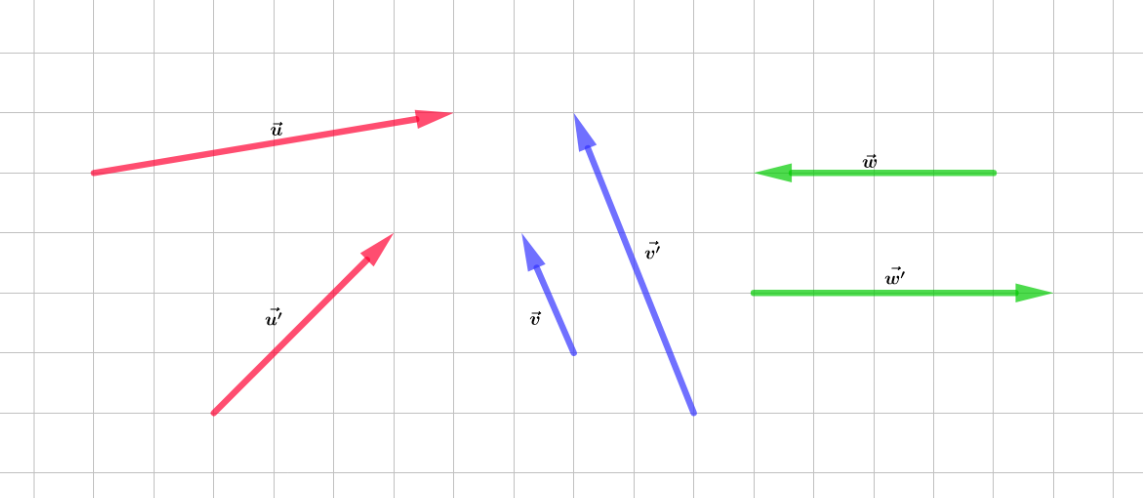
\includegraphics[width=1.0\textwidth]{Vecteurs-DirectionSens.png}
\caption{\textcolor{red}{Les vecteurs $\vec{u}$ et $\vec{u'}$ n'ont pas la même direction}, 
\textcolor{blue}{les vecteurs $\vec{v}$ et $\vec{v'}$ ont même direction et même sens}, 
\textcolor{green}{les vecteurs $\vec{w}$ et $\vec{w'}$ ont même direction, mais un sens opposé}.}
\label{fig:DirectionSens}
\end{figure}

\subsection{Norme d'un vecteur}

Comme souvent en mathématiques, on aime calculer la taille des objets, parce que cela exprime une partie des propriétés d'un objet sous la forme d'un nombre. La longueur d'un vecteur s'appelle la norme.

\begin{de}[Norme d'un vecteur]
  La norme d'un vecteur $\overrightarrow{AB}$ est égale à la longueur du vecteur, c'est à dire à la distance $AB$. On la note $\Vert \overrightarrow{AB} \Vert$
\end{de}

Pour calculer cette distance quand on dispose des coordonnées, il suffit d'utiliser le bon vieux théorème de Pythagore.

\begin{prop}[Norme d'un vecteur dont on connaît les coordonnées]
  Soit $\overrightarrow{u}$ un vecteur de coordonnées $\Coord{x}{y}$, la norme de $\overrightarrow{u}$ est donnée par la formule  \[ \Vert \vec{u} \Vert = \sqrt{x^2+y^2} \]
\end{prop}

Note : La norme est donc toujours positive, et même toujours strictement positive si le vecteur n'est pas nul : $\vec{0}$ est le seul vecteur qui a une norme nulle.

On dispose maintenant des trois éléments caractéristiques d'un vecteur : 

\begin{prop}
  Deux vecteurs non nuls sont égaux si et seulement si ils ont même \textbf{direction}, même \textbf{sens}, et même \textbf{norme}.
\end{prop}

Exercice : dessiner deux vecteurs qui ont même norme mais pas même direction, deux autres même direction et norme mais pas même sens, et enfin deux qui ont même direction et sens mais pas même norme.

On a déjà vu que multiplier un vecteur par un réel $k$ (différent de $0$) conservait la direction du vecteur, et conservait le sens si $k>0$ (et l'inverse si $k<0$). On va voir que la multiplication par un réel a aussi un effet simple sur la norme du vecteur :

\begin{prop}
  soit $k$ un nombre réel et $\vec{u}$ un vecteur,  $\Vert k \times \vec{u} \Vert = |k| \times \Vert \vec{u} \Vert$ 
\end{prop}

On déduit de tout ceci le théorème suivant.

\begin{theo}
 Soient A, B, C et D quatre points du plan.  $ABCD$ est un parallélogramme si et seulement si $\overrightarrow{AB}=\overrightarrow{DC}$.
\end{theo}

Un sens est montré en exercice, la partie "seulement si" est plus ardue : Si ABCD est un parallélogramme, il est facile de montrer que $\overrightarrow{AB}$ et $\overrightarrow{DC}$ ont même norme (car les côtés opposés d'un parallélogramme ont même longueur), 
et ont même direction (car les côtés opposés du parallélogramme), on ne dispose pas vraiment d'argument formel pour dire qu'ils ont même sens, hormis "ça se voit, sinon le quadrilatère ABCD serait croisé".

Attention, le parallélogramme ainsi défini peut être aplati, si les points A,B,C et D sont alignés.



\chapter{Vecteurs et droites}

\subsection{Vecteurs directeurs et équations d'une droite}

Préparez-vous mentalement, cette sous-partie contient des concepts qui lient absolument \textbf{toutes} les notions vues depuis le début de l'année : Ensembles de nombres, fonctions, équations et vecteurs.

\subsubsection{Exprimer une droite du plan dans un repère}

Dans un repère, on peut exprimer presque toutes les droites sous la forme de l'équation \textbf{réduite} $y=ax+b$ (avec $a$ et $b$ des nombre réels). C'est à dire que presque toutes les droites sont des courbes représentatives de fonctions affines, c'est à dire des fonctions de forme $f : x \mapsto ax+b$. 
Mais il nous manque un type de droite si on se contente de cette paramétrisation : les droites verticales ne représentent pas des fonctions (car une fonction a toujours au maximum un point sur une ligne verticale), on ne peut donc les représenter sous la forme de cette équation.

\begin{de}[\'Equation d'un ensemble de points du plan]
    Au même titre qu'un sous-ensemble de la droite réelle peut être exprimée par une ou plusieurs équations, un sous-ensemble du plan peut être exprimé par une équation à deux inconnues, qui expriment les valeurs de (x,y) qui doivent être dessinées : on dessine le point $(x,y)$ si et seulement si le couple $(x,y)$ est solution de l'équation.
\end{de}

Exemples : \begin{itemize}
  \item Sur une droite réelle, l'équation $x \geq 4$ est représentable par tous les points d'abscisse supérieure ou égale à 4 (Cf chapitre sur les intervalle)
  \item Dans le plan, on a vu que toute fonction $f(x)$ admet une représentation graphique, qui est l'ensemble des points $(x,y)$ qui vérifient $y=f(x)$. Par exemple pour la fonction carré, on dessine tous les points tels que l'ordonnée est le carré de l'abscisse, soit $y=x^2$, et seulement ceux-ci.
  \item Toujours dans le plan, une fonction affine $f(x)=ax+b$ a pour représentation graphique une droite, qui admet pour équation réduite $y=ax+b$ : les seuls points dessinés sont les points dont les coordonnées $(x;y)$ vérifient l'équation.
  \item Une droite verticale (c'est à dire parallèle à l'axe des abscisses) a pour équation $x=a$ avec a un certain nombre réel. On voit que la variable $y$ n'apparaît pas dans cette équation.
  \item Dans un repère orthonormé, un cercle autour de l'origine de rayon $1$ est l'ensemble des points situés à une distance de $1$ de l'origine, c'est à dire l'ensemble des points vérifiant $x^2+y^2=1$. C'est l'équation d'un cercle.
\end{itemize}


Attention : Une équation n'est pas unique : on a vu de nombreuses manières d'exprimer une équation sous la forme équivalente.  Pour avoir une seule expression, il faut plus de contraintes


\begin{de}[\'Equation réduite d'une droite]
  Toute droite qui n'est pas parallèle à l'axe des ordonnées dans un repère admet une seule équation de la forme $y=ax+b$ avec $a$ et $b$ des réels. On appelle cette équation l'\underline{équation réduite} de la droite.
\end{de}

Pour obtenir une forme d'équation qui permette d'exprimer \textbf{toutes} les droites du plan, on fait appel à une nouvelle forme d'équation : l'équation cartésienne

\begin{de}[\'Equation cartésienne d'une droite]
  Toute droite dans un repère peut être exprimée comme l'ensemble des points vérifiant une équation de forme $ax+by+c=0$ où $a,b$ et $c$ sont des constantes réelles. 

  Réciproquement, toute équation de cette forme où $a$ et $b$ ne sont pas tous deux égaux à $0$ est l'équation d'une droite du plan.
\end{de}

Exemples :\begin{itemize}
  \item La droite d'équation réduite $y=3x+2$ s'exprime sous la forme $3x-y+2=0$, qui est bien de la forme $ax+by+c=0$
  \item La droite d'équation $x=2$ s'exprime sous la forme $x+0 \times y-2=0$, qui est bien de la forme $ax+by+c=0$
\end{itemize}

Attention : \begin{itemize}
  \item Si $a$ et $b$ sont tous deux nuls, l'équation devient $c=0$ et est donc vérifiée soit par aucun couple $(x,y)$ soit par tous les couples $(x,y)$ du plan. Ce n'est donc pas une droite
  \item Une équation cartésienne n'est pas unique : $2x+3y+4=0$ est une équation équivalente à $4x+6y+8=0$ (On a multiplié les deux termes de l'égalité par 2, ce qui préserve l'équivalence comme vu dans le cours sur les équations)
\end{itemize}

\subsubsection{Vecteur directeur d'une droite}

\begin{de}
Dans le plan, tout vecteur non nul tel que l'image d'un point d'une droite par ce vecteur est un autre point de cette droite est appelé \underline{vecteur directeur} de cette droite.
\end{de}

Une définition alternative est : Soient deux points $A$ et $B$ du plan. Le vecteur $\overrightarrow{AB}$, et donc tout vecteur qui lui est égal est appelé vecteur directeur de la droite $(AB)$

Il existe un lien profond entre vecteur directeur d'une droite et équation cartésienne de la droite :

\begin{prop}
  Soit $\overrightarrow{u} \Coord(a,b)$ un vecteur non nul. Toute droite ayant $\overrightarrow{u}$ pour vecteur directeur 
  admet une équation cartésienne de la forme $bx-ay+c=0$, où $c$ est un nombre réel.
\end{prop}

Remarques: 
  \begin{itemize}
  \item Ici, l'expression est unique car on ne peut plus multiplier l'équation par un réel sinon on perd les a et les b.
  \item \textbf{Attention} : Pour retenir cette formule, il faut se rappeler que l'abscisse du vecteur est devant le $y$ de l'équation, et l'ordonnée devant le $x$. Il y a donc une inversion de l'ordre naturel entre les deux expressions. De plus, un signe moins fait son apparition.
  \end{itemize}

\end{document}

